\section{Cinematica Manipolatore}
L'obiettivo di questa sezione è quello di andare ad illustrare le metodologie che ci hanno consentito di ottenere sia la cinematica diretta per posizione, velocità ed accelerazione che quella inversa.
\\Per proseguire nelle sezioni seguenti andiamo a definire una tabella con i principali parametri del robot:
\begin{table}[h!]
\centering
\begin{tabular}{|c |c |c|} 
 \hline
 Nome & Descrizione  & Valore \\ [0.5ex] 
 \hline\hline
 $l [m]$ & lunghezza link  & 0.25 \\ 
 $m [kg]$ & massa link & 2.9 \\
 $c_m [m]$ & posizione centro di massa & 1.25 \\
 $J_r [kg\cdot m^2]$ & momento d'inerzia baricentrico & $5.22\cdot 10^{-2}$ \\
 $d [m]$ & lunghezza semitelaio & 0.09 \\
 \hline
\end{tabular}
\caption{Parametri manipolatore}
\label{table:1}
\end{table}
Tutti e quattro i link hanno lunghezza, massa, posizione del centro di massa e momento di inerzia uguali, per questo si è deciso di rappresentare i dati una sola volta.
\begin{figure}[ht]
\begin{center}
    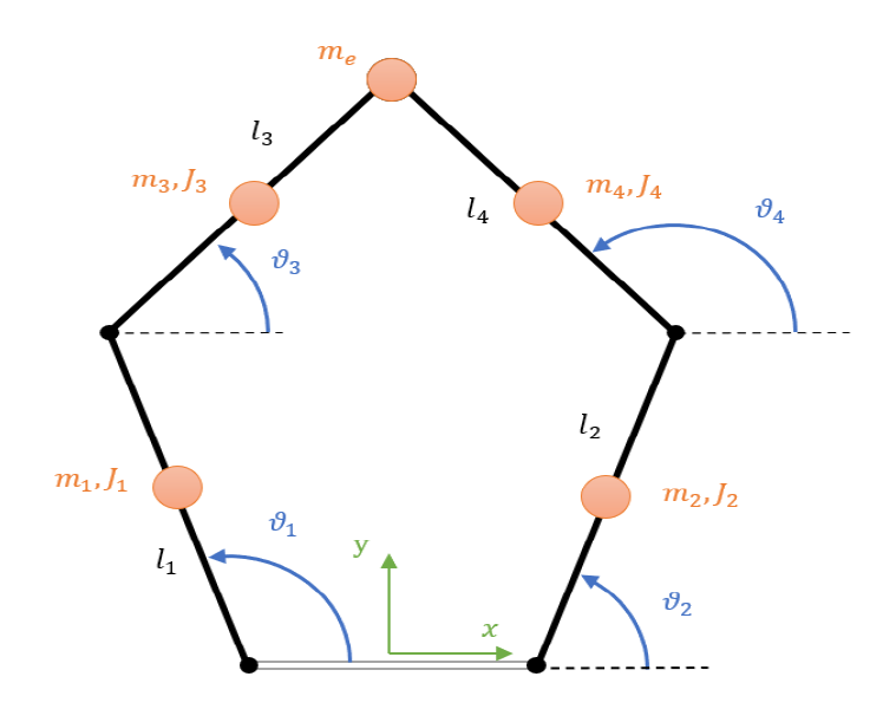
\includegraphics[scale=0.5]{Immagini/Robot2.png}
    \caption{Rappresentazione fisica del robot}
\end{center}
\end{figure}
\subsection{Cinematica Diretta}
La cinematica diretta si occupa di trovare il legame tra i parametri interni del robot e la posa che esso assume, per posa intendiamo posizione ed orientamento. In questa sezione andremo ad analizzare la cinematica diretta di posizione, velocità ed accelerazione.
\subsubsection{Posizione}\label{sec:Cinematica-pos}
Nella cinematica diretta di posizione, a partire dal robot e da $\theta_1$ e $\theta_2$, riusciamo a ricavare la posizione dei link distali (ovvero quelli non motorizzati), il loro angolo, quindi $\theta_3$ e $\theta_4$ e per concludere troviamo anche la posizione $[x,y]$ dell'end-effector.
\\L'approccio al calcolo della cinematica diretta è stato l'utilizzo delle equazioni alle circonferenze:
\begin{equation}
    \begin{cases}
    (x-\frac{l}{2}-l\cos\theta_1)^2+(y-l\sin\theta_1)^2 = l^2 \\
    (x+\frac{l}{2}-l\cos\theta_2)^2+(y-l\sin\theta_2)^2 = l^2
    \end{cases}
\end{equation}
Da questa equazione, andando a sviluppare i calcoli possiamo suddividere in:
\begin{equation*}
    A = l^2 (\sin\theta_2- \sin\theta_1)^2 + (-2\cdot d-l (\cos\theta_2 - \cos\theta_1))^2
\end{equation*}
\begin{equation*}
\begin{aligned}
   B =  -2\cdot l^2 \cdot d (\sin\theta_2-\sin\theta_1)\cdot  (\cos(\theta_2+\theta_1) + l(\sin\theta_2-\sin\theta_1)\cdot   (-2d-l(\cos\theta_2-\cos\theta_1))\\\cdot (-2d-2l\cos\theta_2) - 2l\sin\theta_2\cdot (-2d-l(\cos\theta_2-\cos\theta_1))^2
\end{aligned}
\end{equation*}
\begin{equation*}
\begin{aligned}
    C = l^2\cdot d^2 (\cos\theta_2+\cos\theta_1)^2-l\cdot d (\cos\theta_2+\cos\theta_1)\cdot(-2d-l(\cos\theta_2-\cos\theta_1) ) \\\cdot (-2d-2l\cos\theta_2)+(d^2+2dl\cos\theta_2)\cdot(-2dl(\cos\theta_2-\cos\theta_1))^2
\end{aligned}
\end{equation*}

Da queste espressioni riusciamo facilmente a ricavare la posizione $P = [x,y]$ dell'end-effector, trovando:
\begin{equation}
x = \frac{y\cdot l(\sin\theta_2 - \sin\theta_1)-l\cdot d(\cos\theta_2+\cos\theta_1)}{-2d-l(\cos\theta_2-\cos\theta_1)}, y = \frac{-B + \sqrt{B^2-4AC}}{2A} 
\end{equation}
Per quanto riguarda invece le posizioni dei link distali sono state ottenute nel seguente modo: 
\begin{equation*}
    E_{1X} = -d+l\cdot \cos\theta_1 , E_{1Y}=l\cdot \sin\theta_1
\end{equation*}
e
\begin{equation*}
    E_{2X} = d+ l\cdot \cos\theta_2, E_{2Y} = l\cdot \sin\theta_2
\end{equation*}
E successivamente, gli angoli $\theta_3$ e $\theta_4$, riferiti rispettivamente ad $E_1$ ed $E_2$. Il primo, $\theta_3=$
\begin{equation*}
    \begin{aligned}
    2\cdot tg^{-1}\frac{\sqrt{ (\sin\theta_2 - \sin\theta_1) + \frac{1}{2}((\cos\theta_2 - \cos\theta_1 + \frac{18}{25})^2+(\frac{(\sin\theta_1-\sin\theta_2)^2}{2})^2+(\sin\theta_1-\sin\theta_2)^2)}}{(\cos\theta_2-\cos\theta_1)+\frac{(\cos\theta_2-\cos\theta_1+\frac{18}{25})^2}{2}+\frac{(\sin\theta_1-\sin\theta_2)^2}{2}+\frac{18}{25}}
    \end{aligned}
\end{equation*}
e $\theta_4 =$
\begin{equation*}
    \begin{aligned}
    -2\cdot tg^{-1}\frac{\sqrt{(\sin\theta_2-\sin\theta_1)+(\frac{1}{2}(\cos\theta_2-\cos\theta_1+\frac{18}{25})^2+(\frac{\sin\theta_1-\sin\theta_2)^2}{2})^2+(\sin\theta_1-\sin\theta_2)^2)}}
    {(\cos\theta_1 -\cos\theta_2)+\frac{(\cos\theta_2-\cos\theta_1+\frac{18}{25})^2}{2}+\frac{(\sin\theta_1-\sin\theta_2)^2}{2}+\frac{18}{25}}
    \end{aligned}
\end{equation*}
Quindi, alla fine della cinematica diretta di posizione andiamo ad ottenere la posizione dell'end-effector, la posizione dei link distali e gli angoli dei link distali.
\subsubsection{Velocità}\label{sec:CalcoloVelCin}
La cinematica diretta di velocità ci consente di ricavare la velocità dell'end-effector sulle coordinate x ed y e ci permette di ottenere la jacobiana che lega queste variabili. Partendo da questa equazione
\begin{equation}
    TBD
\end{equation}
Andiamo per semplicità a definire:
\begin{equation*}
    N_{21} = -l\sin\theta_1\cdot (x+d-l\cdot \cos\theta_1 + l\cdot \cos\theta_1\cdot (y-l\sin\theta_1))
\end{equation*}
\begin{equation*}
    N_{22} = -l\cos\theta_2\cdot \frac{(y-l\sin\theta_2\cdot (x+d-l\cos\theta_1))}{x-d-l \cos\theta_2} +l\sin\theta_2\cdot(x+d-l\cos\theta_1)
\end{equation*}
\begin{equation*}
 D_2 = \frac{y-l\sin\theta_2\cdot (x+d-l\cos\theta_1}{x-d-l\cos\theta_2}
\end{equation*}
Fatto questo possiamo andare a definire i parametri della Jacobiana così come segue:
\begin{equation*}
    J_{11} = -\frac{y-l\sin\theta_2}{x-d-l\cos\theta_2}\cdot J_{21}
\end{equation*}
\begin{equation*}
    J_{12} = -\frac{y-l\sin\theta_2}{x-d-l\cos\theta_2}\cdot J_{22} - l\sin\theta_2 + \frac{y-l\sin\theta_2}{x-d-l\cos\theta_2}\cdot l\cos\theta_2
\end{equation*}
\begin{equation*}
    J_{21} = \frac{N_{21}}{D_2}
\end{equation*}
\begin{equation*}
    J_{22} = \frac{N_{22}}{D_2}
\end{equation*}
Andando ad unire le equazioni che abbiamo appena definito troviamo la Jacobiana che lega $\theta_1$ e $\theta_2$:
\begin{equation}
    J = \begin{bmatrix}
    J_{11} & J_{12} \\ J_{21} & J_{22}
    \end{bmatrix}
    \label{eq:J12}
\end{equation}
Possiamo per concludere ricavare la velocità dell'end-effector $\dot{P} = [\dot{x},\dot{y}]$, nel seguente modo:
\begin{equation}
    \dot{x} = J_{11}\cdot \dot{\theta_1} + J_{12}\cdot\dot{\theta_2}, \dot{y} = J_{21}\cdot \dot{\theta_1}+J_{22}\cdot\dot{\theta_2}
\end{equation}
\subsubsection{Accelerazione}
Il processo è simile a quanto visto nelle sezioni precedenti, in questo caso, a partire da tutti i parametri ricavati precedentemente e da $\ddot{\theta_1}$ e $\ddot{\theta_2}$, andiamo a definire le seguenti quantità:
\begin{equation*}
\begin{aligned}
    A_{f} = \dot{x}^2 + 2l\sin\theta_2\cdot\dot{x}\cdot\dot{\theta_2}+(l\sin\theta_2\dot{\theta_2})^2 + (x-d-l\cos\theta_2)\cdot(l\cos\theta_2\dot{\theta_2}+l\sin\theta_2\ddot{\theta_2}) +\\ \dot{y}^2-2l\cos\theta_2\cdot\dot{y}\dot{\theta_2}+(l\cos\theta_2\dot{\theta_2})^2+(y-l\sin\theta_2)\cdot(l\sin\theta_2\dot{\theta_2}^2-l\cos\theta_2\ddot{\theta_2})
    \end{aligned}
\end{equation*}
\begin{equation*}
    \begin{aligned}
    B_{f} = \dot{x}^2+2l\sin\theta_1\cdot\dot{x}\cdot\dot{\theta_1} + (l\sin\theta_1\dot{\theta_1})^2+(x+d.l\cos\theta_1)\cdot(l\cos\theta_1\dot{\theta_1}^2+l\sin\theta_1\ddot{\theta_1})+
    \\ \dot{y}^2 -2l\cos\theta_1\cdot \dot{y}\cdot\dot{\theta_1}+(l\cos\theta_1\dot{\theta_1})^2+(y-l\sin\theta_1)\cdot(l\sin\theta_1\dot{\theta_1}^2-l\cos\theta_1\ddot{\theta_1})
    \end{aligned}
\end{equation*}
Da queste quantità possiamo trovare $\ddot{P} = [\ddot{x},\ddot{y}]$, nel seguente modo:
\begin{equation}
    \ddot{x} = -\frac{\ddot{y}\cdot(y-l\sin\theta_1)}{x+d-l\cos\theta_1}, \ddot{y} = \frac{\frac{B_{f}\cdot(x-d-l\cos\theta_2)}{x+dl\cos\theta_1-A}}{y-l\sin\theta_2-\frac{x-d-l\cos\theta_2}{(x+d-l\cos\theta_1)\cdot(y-l\sin\theta_1)}}
\end{equation}
\subsection{Cinematica inversa}
Il problema della cinematica inversa consiste nel ricavare i valori degli angoli da assegnare ai parametri del robot per riuscire a seguire una determinata legge di moto. L'analisi della cinematica inversa è stata fatta per posizione, velocità ed accelerazione.
\subsubsection{Posizione}
Nella cinematica inversa di posizione, a partire dalla posizione dei link distali, andiamo a ricavare $\theta_1$ e $\theta_2$. Andiamo per semplicità a definire i seguenti parametri:
\begin{equation*}
    p = 2dl + 2xl, e = 2yl, f = x^2+d^2+y^2+2px
\end{equation*}
che serviranno per $\theta_1$
\begin{equation*}
 a = -2dl+2xl, b = 2yl, c = x^2+d^2+y^2-2xd
\end{equation*}
che serviranno per $\theta_2$. 
\\Andiamo a calcolare quindi: 
\begin{equation}
    \theta_1 = 2\arctan\frac{e+\sqrt{p^2+e^2-f^2}}{p+f}
\end{equation}
e
\begin{equation}
    \theta_2 = 2\arctan\frac{b-\sqrt{a^2+b^2-c^2}}{a+c}
\end{equation}
\subsubsection{Velocità}
Per quanto riguarda il calcolo della cinematica inversa in velocità andiamo a prendere l'equazione \ref{eq:J12} e, dopo averla invertita ricaviamo le velocità relative:
\begin{equation}
    \dot{\Theta} = \begin{bmatrix} \dot{\theta_1} \\ \dot{\theta_2}
    \end{bmatrix} = J^{-1} \begin{bmatrix} \dot{x} \\ \dot{y} \end{bmatrix}
\end{equation}
Siamo quindi riusciti ad ottenere le velocità degli angoli a partire dalle velocità all'end-effector.
\subsection{Modellazione su Adams}